\documentclass[letter]{article}

\usepackage{url}
\usepackage{textcomp}
\usepackage{graphicx}
\usepackage{subfig}

\title{gEEProg v2.0 Software User Manual}
\author{\textcopyright\ Mark Chilenski, Matthew D'Asaro 2015\\\url{http://www.dasarodesigns.com/}}

\usepackage{hyperref}

\begin{document}

\maketitle

\section{Overview}
gEEProg is a Python module and GUI program for controlling the 2801Prog, 2006Prog and other D'Asaro Designs EEPROM programmers.
gEEProg is distributed under the terms of the GNU Public License (GPL), a copy of which should have been included with this software.\footnote{\url{http://www.gnu.org/licenses/}}
For the technical details of the programmer itself, refer to the accompanying user and service manual.

\section{Installing the Software}
\subsection{Windows}
An executable (.EXE file) is available at \url{https://github.com/markchil/gEEProg/releases}.
Simply download and unzip this file to a convenient location.
The software is launched by double-clicking the program icon, like any other program.

\subsection{Mac OS X}
An application (.app file) is available at \url{https://github.com/markchil/gEEProg/releases}.
Simply download this file, unzip it and drag gEEProg.app to your Applications folder (or another convenient location).
The software is launched by double-clicking the program icon, like any other program.

\subsection{Linux/Install From Source}
To install from source, you must have the following prerequisites (many of which are already present in most Linux installs):
\begin{description}
	\item[Python version 2.7] Other versions may work but have not been tested. Either use your favorite package manager, or install from \url{https://www.python.org/downloads/}.
	\item[Tkinter] Either use your favorite package manager, or follow the directions here \url{http://tkinter.unpythonic.net/wiki/How_to_install_Tkinter} or here \url{http://www.tkdocs.com/tutorial/install.html}
	\item[pip] Either use your favorite package manager, or follow the directions here \url{https://pip.pypa.io/en/latest/installing.html}
\end{description}
Once you have these prerequisites, installing gEEProg is as simple as running the command ``\texttt{sudo pip install gEEProg}'' (without the quotes).
This will install/upgrade gEEProg's dependencies as needed, then install the gEEProg software itself.
The gEEProg Python module will be placed in your site-packages directory, and can then simply be accessed for use in your own Python scripts with ``\texttt{import gEEProg}''.
The GUI is called ``\texttt{gEEProgGUI}'' and its install location is determined by pip and how your Python installation is structured.
The path to this script will be printed as part of pip's installation process.
Assuming that the directory containing the \texttt{gEEProgGUI} script is part of your shell PATH, you can now launch the software simply by typing ``\texttt{gEEProgGUI}'' from the shell (without the quotes).
If Python 2.7 is not the version you get when typing ``\texttt{python}'' at the shell, then you need to modify the shebang statement at the start of the \texttt{gEEProgGUI} script.
An example of checking for the prerequisites, installing and launching gEEProg on Ubuntu is given in figure~\ref{fig:install}.
\begin{figure}[bh]
	\centering
	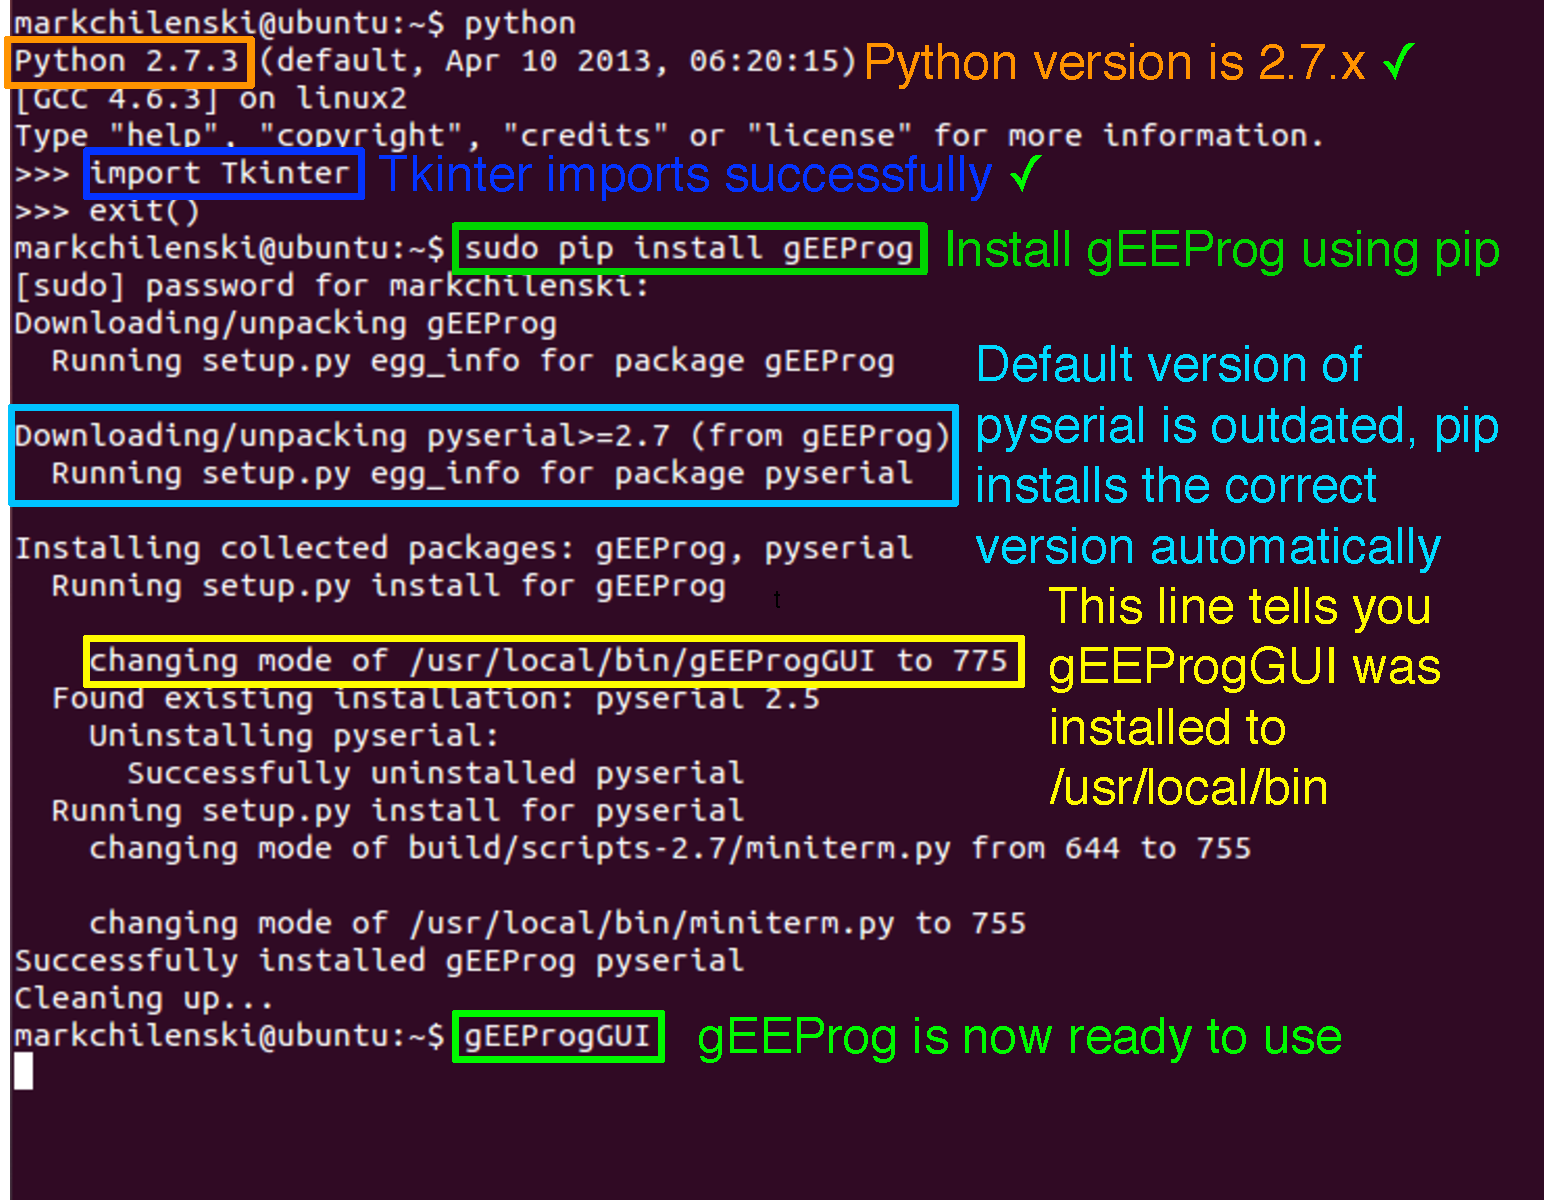
\includegraphics[width=\textwidth]{./graphics/LinuxTutorial}
	\caption{How to check for the prerequisites and install gEEProg from source.}
	\label{fig:install}
\end{figure}

\pagebreak

\section{Connecting to your programmer}
First, connect your programmer to the computer using a serial cable and/or USB-to-serial adapter.
Then, connect the power to your programmer.
Finally, start gEEProg as described above.

When gEEProg first launches, the window will look like figure~\ref{fig:start}.
\begin{figure}
	\centering
	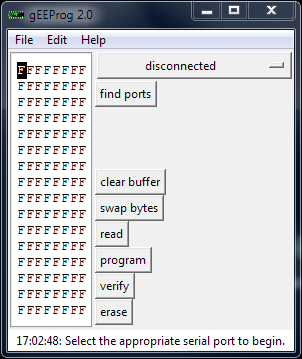
\includegraphics[scale=0.7]{./graphics/start}
	\caption{Starting state of gEEProg.}
	\label{fig:start}
\end{figure}
If you plugged your USB-to-serial adapter in after starting gEEProg, press the ``find ports'' button to refresh the list of available ports.
Then, click the pull down menu (which should say ``disconnected'') and select your programmer's serial port from the list of available options.

Once gEEProg connects to the programmer, the bottom status bar will turn green and some explanatory text will appear -- see figure~\ref{fig:connected}.
\begin{figure}
	\centering
	\subfloat[2801Prog]{
		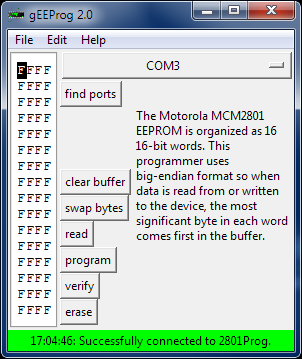
\includegraphics[scale=0.7]{./graphics/2801ProgConnected}
	}
	\subfloat[2006Prog]{
		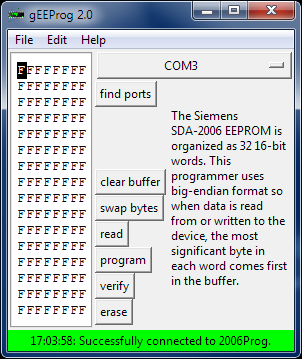
\includegraphics[scale=0.7]{./graphics/2006ProgConnected}
	}
	\caption{gEEProg after successfully connecting to a programmer.}
	\label{fig:connected}
\end{figure}

\subsection*{Troubleshooting}
If gEEProg cannot connect to the programmer, the bottom status bar will turn red.
First, make sure you have selected the correct port.
If you cannot connect on any of the ports, try pulling the power cable from the programmer for a few seconds, then plugging it back in, then trying to connect to the programmer again as described above.

\subsection*{Potential issues on Linux}
If you cannot connect to your serial port on Linux, it may be because you do not have sufficient user permissions.
You can try running gEEProg with sudo to circumvent this, though the best solution is to add your user account to the ``dialout'' group with the command ``\texttt{sudo gpasswd --add [username] dialout}''.

\section{Interacting with the programmer}
\subsection{The buffer}
The buffer on the left side of the window allows you to edit the contents of the memory in hexadecimal.
Use the arrow keys to navigate, or click on a specific nibble to bring the cursor there.
The byte ordering for your particular programmer is described in the text to the right.
To clear the contents of the buffer (i.e., to set each byte to ``\texttt{FF}'') click the ``\textbf{clear buffer}'' button.
To swap the byte order click the ``\textbf{swap bytes}'' button.

\subsection{Reading an EEPROM}
To read the data from the EEPROM chip inserted into the programmer press the ``\textbf{read}'' button.
If the chip is read successfully the bottom status bar will turn green and the contents of the chip will be placed into the buffer for viewing/editing.
If the read fails the status bar will turn red.

\subsection{Programming an EEPROM}
To program the EEPROM chip inserted into the programmer with the contents of the buffer press the ``\textbf{program}'' button.
If the chip is programmed successfully the bottom status bar will turn green.
If the chip fails to program the status bar will turn red.

\subsection{Verifying the contents of an EEPROM}
To verify that the contents of the EEPROM chip inserted into the programmer match the contents of the buffer press the ``\textbf{verify}'' button.
If the contents match the bottom status bar will turn green.
If the contents do not match the status bar will turn red.

\subsection{Erasing an EEPROM}
To erase the EEPROM chip inserted into the programmer press the ``\textbf{erase}'' button.
If the chip's contents have been successfully erased the bottom status bar will turn green.
If the contents were not successfully erased the status bar will turn red.

\section{Advanced features}
\subsection{Saving and opening files with the ``File'' menu}
The ``\textbf{File}'' menu lets you save and open files.
If the file extension is ``.txt'' the file is an ASCII representation of the hexadecimal contents of the buffer, otherwise it is treated as a binary file.
When reading an ASCII file, all non-valid characters are stripped from the input.
This includes spaces and newlines, so you may format your ASCII files to be human-readable.

\subsection{Copying and pasting with the ``Edit'' menu}
The ``\textbf{Edit}'' menu allows you to copy and paste block of hexadecimal data in the buffer.
The ``\textbf{Paste}'' function will paste whatever text you copied last into the buffer starting at the cursor's location.
Non-valid characters will be stripped, so you can copy from a human-readable representation of the desired data.
The ``\textbf{Copy Buffer}'' function will copy the contents of the entire buffer so that you can paste them into another program.

\subsection{Getting help with the ``Help'' menu}
The ``\textbf{gEEProg help...}'' option under the ``\textbf{Help}'' menu will bring up the dialog shown in figure~\ref{fig:help}, which contains links to the websites for both your programmer and the gEEProg software.
\begin{figure}
	\centering
	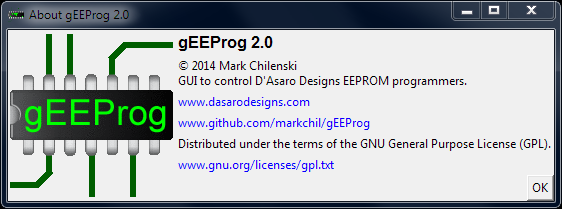
\includegraphics[scale=0.7]{./graphics/help}
	\caption{Help window.}
	\label{fig:help}
\end{figure}

\section{Using the Python API}
gEEProg includes the ``\texttt{gEEProg}'' Python module which gives access to all features of your programmer from within Python.
The main general-purpose functions are:
\begin{description}
	\item[\texttt{enter\_automation\_mode}] Puts the programmer into automation mode such that programs can talk to it properly.
	\item[\texttt{exit\_automation\_mode}] Exits automation mode to allow a user to interact with the programmer directly using a program like minicom.
	\item[\texttt{read\_chip}] Reads the contents of the chip.
	\item[\texttt{verify\_chip}] Verifies that the contents of the chip match the desired data.
	\item[\texttt{program\_chip}] Programs the chip with the desired data.
	\item[\texttt{erase\_chip}] Erases the chip.
\end{description}
Consult the documentation for these functions in the file gEEProg.py, which should have been installed in your site-packages directory.

\end{document}